% !TEX TS-program = pdflatexmk
\documentclass[a4paper,11pt]{article}

\usepackage{Temp_short}
\usepackage[bottom]{footmisc}
\usepackage{commath}
\usepackage{caption} 
\captionsetup[table]{skip=7pt}
\setlength{\jot}{0.3cm}
\allowdisplaybreaks[2]

\newenvironment{Ncenter}{%
  \setlength\topsep{-10pt}
  \setlength\parskip{-10pt}
  \begin{center}
}{%
  \end{center}
}


\bibliographystyle{abbrv}

\newcommand{\kmo}{k_{\mathrm{OT \to O+T}}}
\newcommand{\kOpT}{k_{\mathrm{O+T \to OT}}}
\newcommand{\kmt}{k_{\mathrm{OTE \to OT+E}}}
\newcommand{\kt}{k_{\mathrm{OT+E \to OTE}}}
\newcommand{\kE}{k_{\mathrm{OTE \to OCE}}}
\newcommand{\kD}{k_{\mathrm{OC \to O+C}}}
\newcommand{\vp}{v_{\mathrm{prod}}}
\newcommand{\vd}{k_{\mathrm{T \to \emptyset}}}
\newcommand{\Trel}{T_{\rm{rel}}}
\newcommand{\EC}{EC_{\rm{50}}}
\newcommand{\KdOT}{K_{\mathrm{dOT}}}
\newcommand{\KdOTE}{K_{\mathrm{dOTE}}}
\newcommand{\Trelmin}{T_{\rm{rel,min}}}

\makeatletter 
\renewcommand{\thefigure}{S\@arabic\c@figure}
\renewcommand{\thesection}{~\hspace{-7.5 mm}}
\renewcommand{\thetable}{}
\addto\captionsenglish{\renewcommand{\figurename}{Supplementary Figure}}
\addto\captionsenglish{\renewcommand{\tablename}{Supplementary Table}}

\title{Supplementary Document for Pedersen et al. (2013)}
\author{Lykke Pedersen, \and Peter H Hagedorn, \and Marie Lindholm, \and Morten Lindow}
\date{}

\usepackage{Sweave}
\begin{document}
\Sconcordance{concordance:SuppFile1.tex:SuppFile1.Rnw:%
1 47 1 1 0 8 1 1 2 1 0 2 1 3 0 1 2 14 1 1 4 3 0 1 1 6 0 1 2 1 1 1 30 7 %
1 1 14 1 46 13 1 1 2 1 0 1 3 2 0 1 3 2 0 1 1 1 3 2 0 1 2 1 0 1 1 1 2 1 %
0 1 1 1 2 1 0 1 1 1 2 1 0 1 1 1 2 1 0 1 1 1 2 1 0 1 1 1 2 1 0 1 1 1 2 1 %
0 1 1 1 3 5 0 1 2 8 1 1 7 12 1 1 3 2 0 1 1 1 4 3 0 1 1 1 3 5 0 1 19 11 %
1 1 2 8 0 2 2 1 0 2 1 3 0 1 18 32 1}

\maketitle

This document is the Supplementary Document for the manuscript entitled ``A kinetic model of enzyme recruiting oligonucleotides predicts an optimal affinity and explains why shorter and less affine oligonucleotides can be more potent" and it is a vignette for the R-package ASOmodels.

With the aim of maximising reproducibility, the functions and data used to produce the figures in the main manuscript and this supplementary document are available after installing the ASOmodels package in R.
\begin{Schunk}
\begin{Sinput}
> require(devtools)
> #install_github('ASOmodel',username='lykkep')
> require(ASOmodels)
\end{Sinput}
\end{Schunk}
The ASOmodels package defines and documents the following functions that are used in this document:
\begin{enumerate}
\item \texttt{Trel}
\item \texttt{TrelNO}
\item \texttt{Trelstoc}
\item \texttt{plot.doseresponse}
\item \texttt{EC50}
\item \texttt{EC50NO}
\item \texttt{EC50stoc}
\item \texttt{diffASO}
\item \texttt{pretty10expLP}
\end{enumerate}

\newpage

\tableofcontents

\newpage

%%%%%%%%%%%%%%%%%%%%%%%%%%%%%%%%%%%%%%%%%%%%%%%%%%%%%%%%%%%%%%%%%%%%%%%%%%%%%
\section{Supplementary Figure S1}
The R-function \texttt{Trel()} calculates $\Trel$ as a function of $O_t$ and the set of parameters as in the example below:
\begin{Schunk}
\begin{Sinput}
> #The parameters are in vector-format
> parms <- c(Et = 1,KdOT = 0.3,kOpT = 0.2,KdOTE = 70,kOTpE = 5,	
+            vprod = 0.2,kdegrad = 0.04,alpha=0.1,kcleav = 8)
> Trel(Ot=1,param=parms)
\end{Sinput}
\begin{Soutput}
[1] 0.6538694
\end{Soutput}
\end{Schunk}
$\Trel$ can be calculated for a range of different oligonucleotide concentrations ($O_t$) and from this a dose-response curve is obtained. Supplementary Figure~\ref{fig::Etot} shows the change in the dose-reponse curves as the parameters vary. These plots are produced using \texttt{plot.doseresponse()}.
%%%% FIGURE
\begin{figure}[!b]
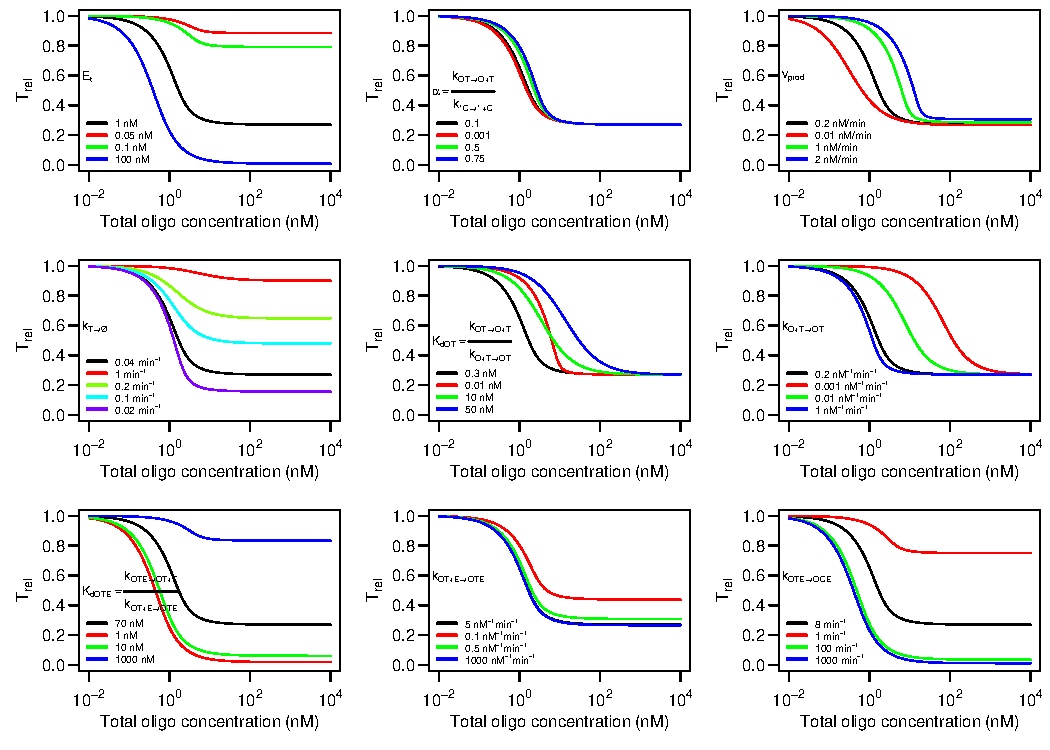
\includegraphics[width=\textwidth]{SuppFile1-S1.pdf}
\caption{Dose-response curves for different values of $E_{t}$, $\alpha$, $\vp$, $\vd$, $\KdOT$, $\kOpT$, $\KdOTE$, $\kt$, and $\kE$ (top,left to bottom,right). Black lines correspond to the parameter values listed in Supplementary Table.}\label{fig::Etot}
\end{figure}


%%%%%%%%%%%%%%%%%%%%%%%%%%%%%%%%%%%%%%%%%%%%%%%%%%%%%%%%%%%%%%%%%%%%%%%%%%%%%
\section{Supplementary Figure S2}
Using the R-function \texttt{drm()} from the drc package (v2.3-0) a dose-response curve is fitted to $\Trel$ as a function of $O_t$ to obtain an $\EC$-value. We are interested in $\EC$ as a function of $\KdOT$. This is calculated through the ASOmodel-function \texttt{EC50()} that takes $\KdOT$ and the set of parameters as input:
\begin{Schunk}
\begin{Sinput}
> EC50(KdOT=0.1,param=parms)
\end{Sinput}
\begin{Soutput}
    EC50 
1.218908 
\end{Soutput}
\end{Schunk}
For a range of $\KdOT$-values, the corresponding $\EC$-values can be calculated. These can be fitted to a parabola using the R-function \texttt{lm()}, see Supplementary Figure S2. 
\begin{Schunk}
\begin{Sinput}
> D1_seq <- 10^seq(-3,3.2,by=0.25)
> ECseq <- sapply(D1_seq,EC50)
> FitPar <- lm(log10(ECseq) ~ log10(D1_seq) + I(log10(D1_seq)^2))
\end{Sinput}
\end{Schunk}
\begin{figure}[!h]
\begin{Ncenter}
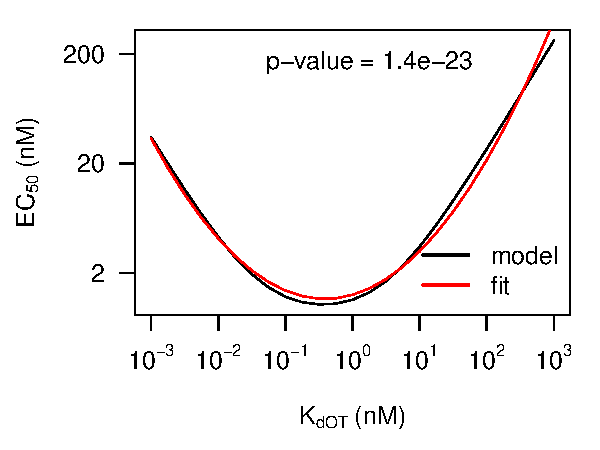
\includegraphics[width=0.6\textwidth]{SuppFile1-S31.pdf}
\end{Ncenter}
\caption{$\EC$ as a function of $\KdOT$ is fitted on a log-log scale to a parabola.}\label{fig::Optfit}
\end{figure}




%%%%%%%%%%%%%%%%%%%%%%%%%%%%%%%%%%%%%%%%%%%%%%%%%%%%%%%%%%%%%%%%%%%%%%%%%%%%%
\section{Supplementary Figure S3}
The stochastic simulation of the model is carried out by use of the \texttt{ssa()} R-function from the GillespieSSA package (v.0.5-4). The inputs to ssa are an initial state vector (x0), which is the initial number of molecules, a propensity vector (a), which denotes the different states of the system, a state-change matrix (nu), which is the change in number of molecule (rows) if a reaction occur (column), the model-parameters (parms) and the final time (tf).
\begin{Schunk}
\begin{Sinput}
> library(GillespieSSA)
> #Model parameters
> parms1 <- c(kOpT = 2E-5,kOTpE =50E-5 ,vprod = 150,  kdegrad = 0.04,		  
+               kcleav = 2, kOT =0.06, kOTE=2, kC = 0.1)
> #Initital state vector
> x0 <- c(Tt=parms1["vprod"]/parms1["kdegrad"],
+         OT=0,OTE=0,E=1e3,O=1e5,OCE=0,OC=0)
> names(x0) <- c('Tt','OT','OTE','E','O','OCE','OC')
> #Propensity vector
> a <-  c("vprod","kOpT*O*Tt","kdegrad*Tt","kOT*OT","kOTE*OTE","kdegrad*OT",
+         "kOTpE*OT*E","kdegrad*OTE","kcleav*OTE","kC*OC","kOTE*OCE" )
> #State-change matrix
> nu <- matrix(0,7,length(a))
> dimnames(nu) <- list(names(x0),a)
> #T
> nu['Tt',c('vprod','kOT*OT')] <- 1
> nu['Tt',c('kOpT*O*Tt','kdegrad*Tt')] <- -1 
> #OT
> nu['OT',c('kOpT*O*Tt','kOTE*OTE')] <- 1
> nu['OT',c('kOT*OT','kOTpE*OT*E','kdegrad*OT')] <- -1
> #OTE
> nu['OTE',c('kOTpE*OT*E')] <- 1
> nu['OTE',c('kOTE*OTE','kdegrad*OTE','kcleav*OTE')] <- -1
> #E
> nu['E',c('kOTE*OTE','kdegrad*OTE','kOTE*OCE')] <- 1
> nu['E',c('kOTpE*OT*E')] <- -1
> #O
> nu['O',c('kOT*OT','kdegrad*OTE','kdegrad*OT','kC*OC')] <- 1
> nu['O',c('kOpT*O*Tt')] <- -1
> #OCE
> nu['OCE',c('kcleav*OTE')] <- 1
> nu['OCE',c('kOTE*OCE')] <- -1
> #OC
> nu['OC',c('kOTE*OCE')] <- 1
> nu['OC',c('kC*OC')] <- -1
> #The Gillespie simulation
> Gillespie <- ssa( x0=x0,a=a,nu=nu,
+       parms = parms1,tf=1E3,method = "ETL")
\end{Sinput}
\end{Schunk}
% Check that $[O]+[OT]+[OTE]+[OCE]+[OC] = O_t$ at all times:
% <<echo=T>>=
% range(rowSums(Gillespie$data[,c('O','OT','OTE','OCE','OC')])-
%         x0['O'])
% @
% Check that $[E]+[OTE]+[OCE] = E_t$ at all times:
% <<echo=T>>=
% range(rowSums(Gillespie$data[,c('OTE','OCE','E')])-x0['E'])
% @
Supplementary Figure~\ref{fig:Trelstoc} shows $\Trel$ from the Gillespie simulation.
\begin{figure}[!h]
\begin{Ncenter}
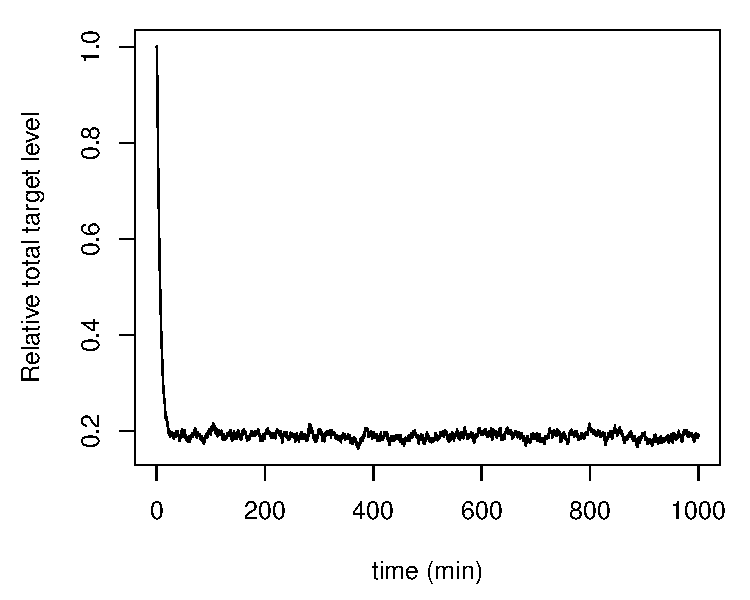
\includegraphics[width=0.6\textwidth]{SuppFile1-Trel.pdf}
\end{Ncenter}
\caption{The time-trace for the relative total target level when the model is simulated stochastically.}\label{fig:Trelstoc}
\end{figure}


%%%%%%%%%%%%%%%%%%%%%%%%%%%%%%%%%%%%%%%%%%%%%%%%%%%%%%%%%%%%%%%%%%%%%%%%%%%%%
\section{Supplementary Figure S4}
After a while the stochastic simulation reaches a plateau. In Supplementary Figure~\ref{fig:Trelstoc} the plateu starts around $50$min. The mean of $\Trel$ within the plateu is calculated through the R-function \texttt{Trelstoc()}. Using this function we can generate dose-response curves (Supplementary Figure~\ref{fig:stocEC50},left). From these $\EC$-values can be calculated using \texttt{EC50stoc()} and they are subsequently plotted as a function of $\kmo$ (Supplementary Figure~\ref{fig:stocEC50},right).
Note that as in the deterministic case (see main manuscript) an optimal affinity is observed.
\begin{Schunk}
\begin{Sinput}
> #### Sequence of k(OT -> O+T) values
> lseq <- c(1,2.5,5,7.5)
> lKOT <- c(1E-3*lseq[-1],1E-2*lseq,1E-1*lseq)
> #### Generation of dose-response curves
> DRcurve <- lapply(lKOT,function(ki){ 
+             sapply(10^seq(2.5,6,by=0.2),
+                    function(i) Trelstoc(i,kOT=ki)$Tstat)})
> DRc <- lapply(DRcurve,function(x) x[,!is.na(x[3,])] )
> #### Calculation of EC50
> EC50_lKOT <- sapply(1:length(DRc),
+               function(x){EC50stoc(DRc[[x]][2,],DRc[[x]][1,])})
\end{Sinput}
\end{Schunk}
\begin{figure}[!h]
\begin{Ncenter}
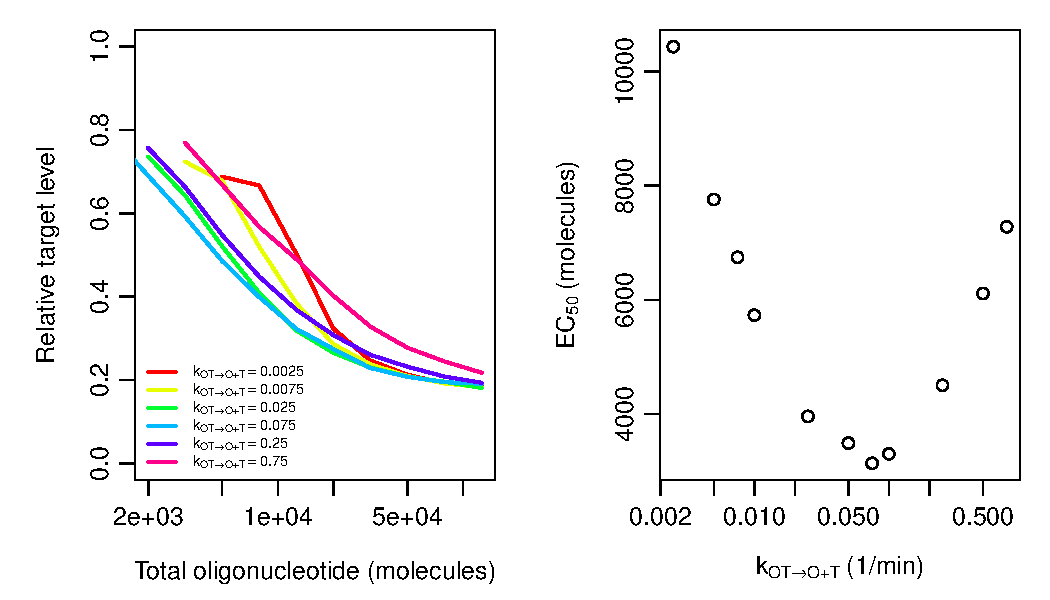
\includegraphics[width=\textwidth]{SuppFile1-EC50.pdf}
\end{Ncenter}
\caption{Left: Dose-response curves for various values of $\kmo$ (compare to Supplementary Figure S1,middle). Right: $\EC$ as a function of $\kmo$. A high value of $\kmo$ corresponds to a low affinity.}\label{fig:stocEC50}
\end{figure}
\newpage


%%%%%%%%%%%%%%%%%%%%%%%%%%%%%%%%%%%%%%%%%%%%%%%%%%%%%%%%%%%%%%%%%%%%%%%%%%%%%
\section{Supplementary Figure S5}
\begin{figure}[!h]
\begin{Ncenter}
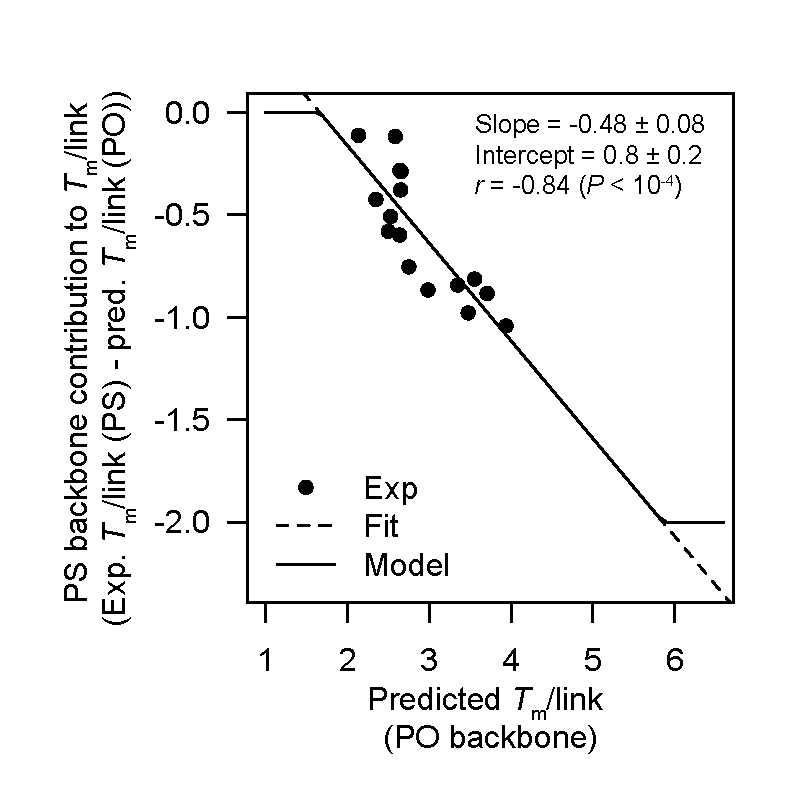
\includegraphics[width=0.65\textwidth]{SuppFig_PS.pdf}
\end{Ncenter}
\caption{The effect on $T_m$ of a phosphorothioate backbone was estimated using published data from Ref. \cite{Hashem:1998kf}.}\label{fig:figPS}
\end{figure}


%%%%%%%%%%%%%%%%%%%%%%%%%%%%%%%%%%%%%%%%%%%%%%%%%%%%%%%%%%%%%%%%%%%%%%%%%%%%%
\section{Supplementary Figure S6}
\begin{figure}[!h]
\begin{Ncenter}
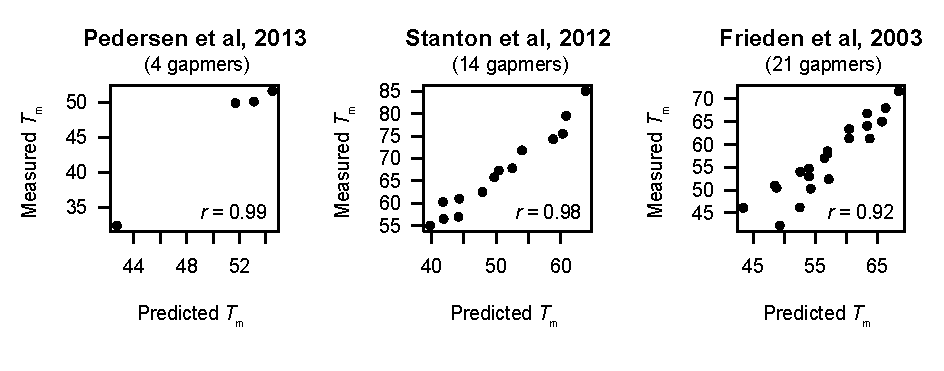
\includegraphics[width=\textwidth]{SuppFigS3.pdf}
\end{Ncenter}
\caption{Measured melting temperature versus predicted melting temperature. There are clear correlations ($r > 0.92$, $P < 0.01$, Pearson's correlation) between predicted and measured $T_m$. Pedersen et al: 4 LNA-modified oligonucleotides targeting apolipoprotein B (this work), Stanton et al: 14 LNA-modified oligonucleotides targeting the glucocorticoid receptor \cite{Stanton:2012fu}. Frieden et al: 21 LNA-modified oligonucleotides targeting the luciferase firefly gene \cite{Frieden:2003er}. Melting curves were recorded with a Perkin Elmer spectrophotometer. Oligonucleotide and its complementary RNA, both at 1.5$\mu M$, were dissolved in buffer (20mM phosphate buffer, 100mM NaCl, 0.1nM EDTA, pH 7). Samples were denatured at $95^\circ$C for 3min and slowly cooled to $20^\circ$C prior to measurements. Melting curves were recorded at 260nm using a heating rate of 1$^\circ$C/min, a slit of 2nm and a response of 0.2s. From this, $T_m$-values were obtained from the maxima of the first derivatives of the melting curves.}\label{fig:figTm}
\end{figure}

\newpage
\bibliography{ASOmodels}


\end{document}
